\section{Diagnosis: Where the Recoverable IoU Goes}
\label{sec:diagnosis}

\subsection{Setting and notation}

A training-free RIS pipeline is a pair $(\mathcal{P}, S)$. The proposer
$\mathcal{P}$ maps an image $x$ to a pool of $N$ candidate masks
$M=\{m_1,\dots,m_N\}$. The scorer $S$ maps a mask, the image and an expression
$e$ to a scalar. The pipeline returns $m_{\hat\imath}$ with
$\hat\imath = \arg\max_i S(m_i, x, e)$; the released HybridGL pipeline instead
returns an argmax over a guidance-weighted score restricted to a small
candidate set, which §\ref{sec:confinement} makes precise.

For a ground-truth mask $g$ we define the \emph{oracle} proposal
$\imath^\star = \arg\max_i \mathrm{IoU}(m_i, g)$ and the \emph{oracle gap}
\[
  \Gamma \;=\; \mathrm{IoU}(m_{\imath^\star}, g) \;-\; \mathrm{IoU}(m_{\hat\imath}, g).
\]
$\Gamma$ is a property of $(x, g, M)$ and the selector only: the oracle itself
does not depend on $S$. The oracle IoU measures what the pool makes available;
$\Gamma$ measures what the selector discards.

\subsection{An error taxonomy of the oracle gap}

We classify each expression by the geometric relation between the returned
mask and the oracle mask, using only mask geometry and the ground truth:

\begin{itemize}
\item \textbf{correct} --- the returned mask already has $\mathrm{IoU} \ge 0.5$
with $g$;
\item \textbf{under-segmentation} --- the returned mask is a strict subset of
the oracle (the oracle is a strict superset and covers $\ge 95\,\%$ of it);
\item \textbf{over-segmentation} --- the oracle is a strict subset of the
returned mask;
\item \textbf{wrong-instance} --- the two masks are near-disjoint,
$\mathrm{IoU} < 0.1$, and neither contains the other;
\item \textbf{boundary} --- overlapping, neither containing the other, and not
near-disjoint.
\end{itemize}

The classes are disjoint and exhaustive by construction. Containment is
evaluated before the disjointness test, so a tiny mask inside a large one is
never miscounted as a separate instance.

\begin{table}[t]
\caption{Error taxonomy of the oracle gap. Each cell is
\emph{prevalence}\,/\,\emph{share of total gap mass}. Full RefCOCO validation
split, 10{,}834 expressions, oracle mIoU 0.8221 in both columns. Under-seg.\ =
under-segmentation; over-seg.\ = over-segmentation.}
\label{tab:taxonomy}
\centering
\small
\begin{tabular}{lcc}
\toprule
& \textbf{unguided argmax} & \textbf{released guidance} \\
& (mIoU 0.3518) & (mIoU 0.4482) \\
\midrule
correct              & 0.371 / 0.022 & 0.478 / 0.027 \\
under-seg.           & 0.109 / 0.143 & 0.108 / 0.176 \\
over-seg.            & 0.011 / 0.010 & 0.016 / 0.019 \\
\textbf{wrong-instance} & \best{0.493 / 0.822} & \best{0.380 / 0.774} \\
boundary             & 0.015 / 0.003 & 0.018 / 0.004 \\
\bottomrule
\end{tabular}
\end{table}

Table~\ref{tab:taxonomy} and Fig.~\ref{fig:taxonomy} give the result. At the
unguided operating point the selector discards 82.2\,\% of the recoverable IoU
on wrong-instance failures; at the released operating point, where the guidance
modules are active, 77.4\,\%. Under-segmentation --- the class addressed by
mask merging, mask refinement, and containment-based remedies --- accounts for
14.3\,\% and 17.6\,\% respectively. Over-segmentation is negligible at every operating point
($\le 1.9\,\%$), which is itself informative: the selector essentially never
errs by returning a mask that contains the referent.

The wrong-instance class is not a small-mask artefact. Its mean returned IoU
against ground truth is $0.006$ while its mean oracle IoU is $0.809$: the
selector is choosing an object, not a fragment, and choosing the wrong one.

\subsection{Wrong-instance is spatial reference failure}
\label{sec:spatial}

Classifying the expressions lexically shows what the wrong-instance cases are
made of. 84\,\% of them contain a spatial word (\emph{left}, \emph{right},
\emph{middle}, \emph{top}, \emph{second from\,\dots}) against 67\,\% of the
split overall under the same broad lexical probe; the relation parser used by
the operator (§\ref{sec:method}) is narrower than that probe and fires on
57.4\,\% of the split, which is the coverage figure used in
Table~\ref{tab:cross}. Typical members are \emph{``left green pot''}, \emph{``person
second from left''}, \emph{``right bear''}, \emph{``horse of left''}. The
referent is also not buried deep in the ranking: at the unguided operating
point its median score-rank is 4.

\begin{figure}[t]
\centering
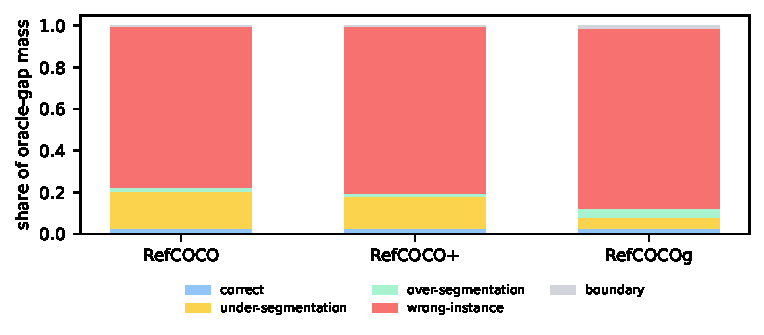
\includegraphics[width=\columnwidth]{figures/taxonomy.pdf}
\caption{Oracle-gap taxonomy on full RefCOCO val, at the unguided argmax
operating point (left) and at the released HybridGL operating point (right).
Solid bars: share of the total recoverable IoU. Hatched bars: prevalence.
Wrong-instance selection dominates the gap mass at both operating points,
although the guidance modules reduce its prevalence; under-segmentation, which
granularity remedies target, carries a small and operating-point-dependent
share.}
\label{fig:taxonomy}
\end{figure}

\subsection{Why the released guidance cannot repair it}
\label{sec:confinement}

HybridGL's guidance modules are not absent, they are \emph{confined}. The
released implementation computes a semantic score per proposal, keeps
$\mathrm{topk}(\text{score}, k_1{=}3)$, forms a spatial-relationship term and a
GEM attention $\times$ position-mask coherence term for those three, and
returns
\begin{equation}
  \hat\imath \;=\; \operatorname*{arg\,max}_{i \in \mathcal{T}}\;
  (1-\alpha)\, r_i \;+\; \alpha\, c_i ,
  \qquad \mathcal{T} = \mathrm{topk}(\text{score}, 3),
  \label{eq:released}
\end{equation}
with $r_i$ the relationship term, $c_i$ the coherence term and $\alpha=0.6$.
The candidate set $\mathcal{T}$ is fixed before any spatial reasoning happens,
so no amount of relation or coherence modelling can return a proposal outside
it.

\begin{table}[t]
\caption{Confinement of the released guidance on full RefCOCO val (10{,}834
expressions, oracle mIoU 0.8221). ``Category score'' is the same scorer
reading the expression with its spatial vocabulary removed.}
\label{tab:confinement}
\centering
\small
\begin{tabular}{lc}
\toprule
measurement & value \\
\midrule
oracle inside released top-3 (all expressions)      & 0.639 \\
oracle inside released top-3 (wrong-instance)       & \best{0.302} \\
mean score-rank of the oracle (wrong-instance)      & 9.1 \\
oracle inside category-score top-8 (wrong-instance) & \best{0.701} \\
mIoU of a perfect chooser inside released top-3     & 0.5812 \\
mIoU actually achieved                              & 0.4482 \\
\bottomrule
\end{tabular}
\end{table}

Table~\ref{tab:confinement} quantifies the consequence. Two numbers matter.
First, the confinement costs real accuracy: a perfect chooser restricted to
the set the released pipeline already computes would reach 0.5812 mIoU against
the 0.4482 it achieves --- $+13.3$ mIoU is available \emph{inside the released
candidate set}. Second, the confinement is what blocks the repair: on the
wrong-instance failures the referent is inside $\mathcal{T}$ only 30.2\,\% of
the time, but inside the top-8 of the category score 70.1\,\% of the time.

The category score is the same frozen text encoder evaluated on the expression
after its spatial vocabulary has been removed --- \emph{``left green pot''}
becomes \emph{``green pot''}. It is a probe for \emph{which objects are
candidates at all}, deliberately stripped of the part of the expression that
the existing score already handles poorly. That a lexical edit of the prompt
produces a better candidate set than the prompt itself is the empirical content
of this section.
